%% ID: two_rods
%% TITLE: Two rods and a hinge
%% TYPE: question
%% QUESTIONTYPE:  numerical
%% CONCEPTS: forces, moments, newtonii, friction
%% VIDEOS: 
%% LEVEL: 5
%% TOPIC: mechanics/statics
%% ORDER: 8

\begin{problem}[A1986FMIIQ3l]
{\question{Two uniform rods AB and CD, each of length \vari{6a} and mass \vari{m} are freely hinged together at H where AH=CH=\vari{2a}. The rods rest in equilibrium with A and C on a rough horizontal table and at a distance \vari{2a} apart. Particles of mass \vari{5m} and \vari{4m} are suspended from B and D respectively. The setup is shown in Figure \ref{fig:Statics_picnic_table_question} below. 
\begin{figure}[h]
	\centering
	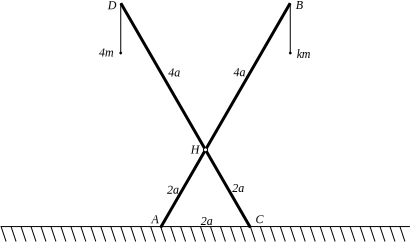
\includegraphics[width=12cm]{../../../figures/Statics_picnic_table_question.eps}
	\caption{The two rods with the masses suspended from them}
	\label{fig:Statics_picnic_table_question}
\end{figure}
\\
The coefficient of friction between each rod and the table is \vari{\mu}. Find the least possible value of \vari{\mu}.}
}
{\textit{Used with permission from UCLES, A Level Further Maths, Syllabus A, June 1986, Paper II, Question 3}}
{\answer{$\mu\ge\frac{10}{9}\sqrt 3$}
Figure \ref{fig:Statics_picnic_table_answer} shows the forces acting on the system:
\begin{figure}[h]
\centering
\includegraphics[width=12cm]{Statics_picnic_table_answer}
\caption{}
\label{fig:Statics_picnic_table_answer}
\end{figure}
\\
As usual in order to solve this equilibrium problem we will need to resolve forces and take moments. First, consider the vertical forces acting. We find:
\begin{align*}
N_A+N_C=4mg+mg+mg+5mg=11mg
\end{align*}
and then balancing horizontal forces
\begin{align*}
F_A=F_C
\end{align*}
Now taking moments on rod $AB$, about the hinge $H$:
\begin{align*}
(4a)5mg\sin{30}+(a)mg\sin{30}+(2a)N_A\sin{30}&=(2a)F_A\cos{30} \\
\Rightarrow 10mg+\frac{1}{2}mg+N_A&=\sqrt 3\: F_A
\end{align*}
And lastly the moments on rod $BC$ about the hinge:
\begin{align*}
(4a)4mg\sin{30}+(a)mg\sin{30}+(2a)N_C\sin{30}&=(2a)F_C\cos{30} \\
\Rightarrow 8mg+\frac{1}{2}mg+N_C=\sqrt 3 \: F_C&=\sqrt 3\: F_A
\end{align*}
These are the four simultaneous equations we need to solve for our four unknowns. Equating the two expressions for $\sqrt 3 \: F_A$ we find
\begin{align*}
 8mg+\frac{1}{2}mg+N_C&=10mg+\frac{1}{2}mg+N_A \\
\Rightarrow -2mg+N_C&=N_A \\
\Rightarrow -2mg+2N_C&=N_A+N_C  
\end{align*}
We have an expression for $N_A+N_C$ that we can substitute in:
\begin{align*}
-2mg+2N_C&=11mg \\
\Rightarrow N_C&=\frac{13}{2}mg
\end{align*}
and therefore we can find an expression for $N_A$:
\begin{align*}
N_A=11mg-N_C \\
\Rightarrow N_A&=11mg-\frac{13}{2}mg \\
\Rightarrow N_A&=\frac{9}{2}mg
\end{align*}
And finally we can find $F_A$ and $F_C$:
\begin{align*}
\sqrt 3 \: F_A=\sqrt 3 \: F_C&=\frac{21}{2}mg+N_A \\
\Rightarrow \sqrt 3 \: F_A&=\frac{30}{2}mg\\
\Rightarrow F_A&=\frac{30mg}{2\sqrt3}
\end{align*}
We also know that $F_A\le\mu N_A$ and $F_C\le \mu N_C$. Because the normal reaction force at $A$ will be greater than that at $C$, the least possible of $\mu$ will come from point $A$ since $F_A=F_B$ but $N_A>N_C$. Therefore we can say 
\begin{align*}
\mu&\ge\frac{F_A}{N_A} \\
\Rightarrow \mu&\ge\frac{mg(30)}{2\sqrt 3}\cdot\frac{2}{mg(9)} \\
\Rightarrow \mu&\ge\frac{10}{9}\sqrt 3
\end{align*} 
}
\end{problem}